%!TEX root = ../bgsu21.tex

\begin{frame}{Operations at odd primes}

	Steenrod also defined operations
	\[
	\beta^{\varepsilon} P_k \colon H^\bullet(X; \Fp) \to H^\bullet(X; \Fp).
	\]

	\pause How to generalize the cup-$i$ products to cochain level operations for all $p$?

	\smallskip \pause
	\begin{enumerate}
		\item Construct $\Sym_p$-equivariant chain maps
		\[
		\rE \Sym_p \otimes \gchains \to \gchains^{\otimes p}
		\]
		for $\rE \Sym_p$ a resolution of $\Z$ by free $\Z[\Sym_p]$-modules.
		\vspace*{10pt} \pause
		\item Identify chains in $\rE \Sym_p$ whose orbits in $(\rE \Sym_p)_{\Sym_p} = \rB \Sym_p$ represent mod-$p$ homology classes.
	\end{enumerate}

	\medskip \pause	The first step is systematized using the theory of \textit{operads}.

	\smallskip \pause The second uses that $\bC_p \to \Sym_p$ induces a surjection in mop-$p$ homology.
\end{frame}

\begin{frame}[fragile]{Canonical example of operad}
	\pause Let $C$ be a chain complex, consider the set
	\[
	\End^C = \left\{ \Hom(C, C^{\otimes r}) \right\}_{r \geq 1}.
	\]

	\pause	Ii is equipped with the structure of an operad:
	\begin{enumerate}
		\item A left action of $\Sym_r$ on $\End^C(r)$, \pause
		\item Composition chain maps
		\[
		\begin{tikzcd}[column sep=small, row sep=tiny]
			\circ_i \colon &[-10pt] \End^C(r) \otimes \End^C(s) \arrow[r] & \End^C(r+s-1) \\
			& f \otimes g \arrow[r, |->] & (1 \otimes \cdots \otimes g \otimes \cdots \otimes 1) \circ f
		\end{tikzcd}
		\]
	\end{enumerate}
	satisfying forms of equivariance, associativity, and unitality.

	\pause \vspace*{10pt}

	\textcolor{pblue}{Slogan:} Abstract groups are to automorphism groups like operads are to these coendomorphism operads.
\end{frame}

\begin{frame}{A graphical example}
	\pause \vspace*{-5pt} Consider the directed labeled graph
	\[
	\begin{tikzpicture}[scale=.5]
		\draw (0,0)--(0,.75);
		\draw (0,0)--(.5,-.5);
		\draw (0,0)--(-.5,-.5);
		\node[scale=.5] at (-.5,-.75){1};
		\node[scale=.5] at (.5,-.75){2};
	\end{tikzpicture}
	\]

	\pause \vspace*{-5pt} Define $\cA(r)$ to be the free module generated by all (relabeled) ``graftings"
	\[
	\begin{tikzpicture}[scale=.75]
		\draw (-.5,1)--(.5,1)--(.5,0)--(-.5,0)--(-.5,1);
		\node[scale=.75] at (0,.5){$\Gamma$};

		\draw (0,1)--(0,1.25);
		\node[scale=.5] at (0,1.5){1};

		\draw (-.5,0)--(-.5,-.25);
		\node[scale=.5] at (-.5,-.5){1};
		\draw (.5,0)--(.5,-.25);
		\node[scale=.75] at (.5,-.5){$r$};
		\node[scale=.75] at (0,-.5){$\cdots$};
	\end{tikzpicture}
	\quad
	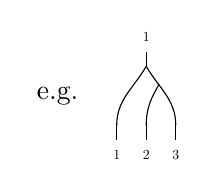
\begin{tikzpicture}[scale=.75]

		\node at (-1.5, 0.5){e.g.};
		\draw (0,1)--(0,1.25);
		\node[scale=.5] at (0,1.5){1};

		\draw (0,1) to  [out=-120,in=90] (-.5,0);
		\draw (0,1) to  [out=-60,in=90] (.5, 0);
		\draw (.22,.7) to  [out=-120,in=90] (0,0);

		\draw (-.5,0)--(-.5,-.25);
		\node[scale=.5] at (-.5,-.5){1};
		\draw (0,0)--(0,-.25);
		\node[scale=.5] at (0,-.5){2};
		\draw (.5,0)--(.5,-.25);
		\node[scale=.5] at (.5,-.5){3};
	\end{tikzpicture}
	\vspace*{-5pt}
	\]

	\smallskip \pause An operad morphism $\cA \to \Hom^C$ is determined by the assignment
	\[
	\coproduct \mapsto \Delta
	\]
	of an element $\Delta \in \Hom(C, C^{\otimes 2})$, i.e., of a (non-necessarily coassociative or cocommutative) coalgebra structure on $C$.
\end{frame}

\begin{frame}[fragile]{$E_\infty$-coalgebras}
	Let $\cO$ be an operad, a $\cO$-\textit{coalgebra} on $C$ is a structure preserving
	\[
	\cO \to \End^C.
	\]
	\pause This corresponds to compatible equivariant maps $\cO(r) \otimes C \to C^{\otimes r}$.

	\medskip \pause	Compare with Steenrod's	\vspace*{-5pt}
	\[
	\begin{tikzcd}[%
		row sep=tiny,
		column sep = small,
		,row sep = 0ex
		,/tikz/column 1/.append style={anchor=base east}
		,/tikz/column 2/.append style={anchor=base west}
		]
		\cW(2) \arrow[r] & \Hom \left( \gchains, \gchains^{\otimes 2} \right) \\
		e_i \arrow[r, |->] & \Delta_i
	\end{tikzcd}
	\]

	\pause \vspace*{-10pt}
	\begin{definition}
		An operad $\cO$ is said to be $E_\infty$ if each $\cO(r)$ is a free resolution of $\Z$ by $\Z[\Sym_r]$-modules
	\end{definition}

	\smallskip \pause Coalgebras over $E_\infty$-operads are thought of as being coassociative and cocommutative up to coherent homotopies.
\end{frame}

\begin{frame}{A finitely presented model}
	\pause Consider the directed labeled graphs
	\[
	\begin{tikzpicture}[scale=.5]
		\draw (0,0)--(0,.75);
		\draw (0,0)--(.5,-.5);
		\draw (0,0)--(-.5,-.5);
		\node[scale=.5] at (-.5,-.75){1};
		\node[scale=.5] at (.5,-.75){2};
	\end{tikzpicture}
	\qquad
	\begin{tikzpicture}[scale=.5]
		\draw (0,0)--(0,-.75);
		\draw (0,0)--(.5,.5);
		\draw (0,0)--(-.5,.5);
		\node[scale=.5] at (-.5,.75){1};
		\node[scale=.5] at (.5,.75){2};
	\end{tikzpicture}
	\vspace*{-10pt}
	\]

	Define $\Med(s, r)_n$ as the free module generated by all (relabeled) ``graftings" and disjoint unions of these of the form
	\[
	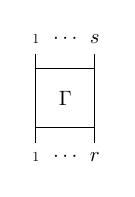
\begin{tikzpicture}[scale=.75]
		\draw (-.5,1)--(.5,1)--(.5,0)--(-.5,0)--(-.5,1);
		\node[scale=.75] at (0,.5){$\Gamma$};

		\draw (-.5,1)--(-.5,1.25);
		\node[scale=.5] at (-.5,1.5){1};
		\draw (.5,1)--(.5,1.25);
		\node[scale=.75] at (.5,1.5){$s$};
		\node[scale=.75] at (0,1.5){$\cdots$};

		\draw (-.5,0)--(-.5,-.25);
		\node[scale=.5] at (-.5,-.5){1};
		\draw (.5,0)--(.5,-.25);
		\node[scale=.75] at (.5,-.5){$r$};
		\node[scale=.75] at (0,-.5){$\cdots$};
	\end{tikzpicture}
	\vspace*{-5pt}
	\]
	with $n$-copies of the \product.
	\pause The boundary map is obtained by removing their incoming strands one at the time: \vspace*{-5pt}
	\[
	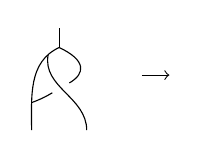
\begin{tikzpicture}[scale=.35]
		\draw (1,3.7) to (1,3);
		\draw (1,3) to [out=205, in=90] (0,0);
		\draw [shorten >= 0cm] (.6,2.73) to [out=-100, in=90] (2,0);
		\draw [shorten >= .15cm] (1,3) to [out=-25, in=30, distance=1.1cm] (1,1.5);
		\draw [shorten <= .1cm] (1,1.5) to [out=210, in=20] (0,1);

		\draw[->] (4,2) to (5,2);
	\end{tikzpicture}
	\qquad %%%%%%%%%%
	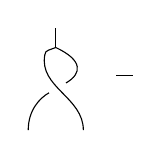
\begin{tikzpicture}[scale=.35]
		\draw (1,3.7) to (1,3);
		\draw (1,3) to [out=205, in=90] (.6,2.73);
		\draw [shorten >= 0cm] (.6,2.73) to [out=-100, in=90] (2,0);
		\draw [shorten >= .15cm] (1,3) to [out=-25, in=30, distance=1.1cm] (1,1.5);
		\draw [shorten <= .1cm] (1,1.5) to [out=210, in=90] (0,0);

		\draw (3.2,2) to (3.8,2);
	\end{tikzpicture}
	\quad %%%%%%%%%%
	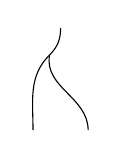
\begin{tikzpicture}[scale=.35]
		\draw (1,3.7) to [out=-90, in=45] (.6,2.73);
		\draw (.6,2.73) to [out=225, in=90] (0,0);
		\draw [shorten >= 0cm] (.6,2.73) to [out=-100, in=90] (2,0);
	\end{tikzpicture}
	\]
\end{frame}

\begin{frame}{A finitely presented model}
	\begin{theorem}[Med.]
		The operad $\UMed$ defined by $\UMed(r) = \Med(1,r)$ is $E_\infty$.
		\medskip\pause
		The collection of maps $\gchains(\gsimplex^n) \to \gchains(\gsimplex^n)^{\otimes r}$ obtained from compositions of
		\begin{align*}
			\Delta &\colon \gchains(\gsimplex^n) \to \gchains(\gsimplex^n)^{\otimes 2}
			\qquad \text{(AW diagonal)} \\
			\ast &\colon \gchains(\gsimplex^n)^{\otimes 2} \to \gchains(\gsimplex^n)
			\qquad \text{(Join map)}
		\end{align*}
		defines an $E_\infty$-coalgebra on simplicial chains.
	\end{theorem}

	\pause

	\qquad \qquad \scalebox{0.7}{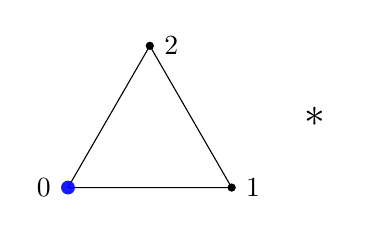
\begin{tikzpicture}[scale=.6]
\coordinate (A) at (210:2);
\coordinate (B) at (-30:2);
\coordinate (C) at (90:2);

\draw[draw=black] (A) -- (B) -- (C) -- (A);

\node[circle,fill=blue, opacity=.9, inner sep=0pt,minimum size=5pt, label=left:{0}] (a) at (A) {};
\node[circle,fill=black,inner sep=0pt,minimum size=3pt, label=right:{$1$}] (a) at (B) {};
\node[circle,fill=black,inner sep=0pt,minimum size=3pt, label=right:{$2$}] (a) at (C) {};

\node[scale=1.5] at (3.5,0.5) {$\ast$};
\end{tikzpicture}
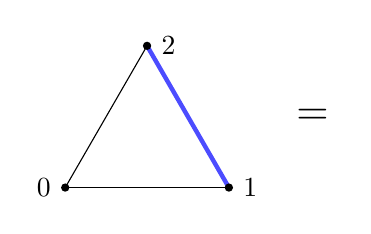
\begin{tikzpicture}[scale=.6]
\coordinate (A) at (210:2);
\coordinate (B) at (-30:2);
\coordinate (C) at (90:2);

\draw[draw=blue,  ultra thick, draw opacity=.7] (B) -- (C);
\draw[draw=black] (C) -- (A);
\draw[draw=black] (A) -- (B);

\node[circle,fill=black,inner sep=0pt,minimum size=3pt, label=left:{$0$}] (a) at (A) {};
\node[circle,fill=black,inner sep=0pt,minimum size=3pt, label=right:{$1$}] (a) at (B) {};
\node[circle,fill=black,inner sep=0pt,minimum size=3pt, label=right:{$2$}] (a) at (C) {};

\node[scale=1.5] at (3.5,.5) {=};
\end{tikzpicture}
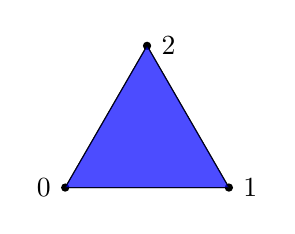
\begin{tikzpicture}[scale=.6]
\coordinate (A) at (210:2);
\coordinate (B) at (-30:2);
\coordinate (C) at (90:2);

\draw[draw=black] (A) -- (B) -- (C) -- (A);

\node[circle,fill=black,inner sep=0pt,minimum size=3pt, label=left:{$0$}] (a) at (A) {};
\node[circle,fill=black,inner sep=0pt,minimum size=3pt, label=right:{$1$}] (a) at (B) {};
\node[circle,fill=black,inner sep=0pt,minimum size=3pt, label=right:{$2$}] (a) at (C) {};

\draw[draw, fill=blue, opacity=.7] (A) -- (B) -- (C) -- (A);
\end{tikzpicture}}

	\medskip\pause

	Also, versions for: \par
		\qquad \textcolor{pblue}{cubical} (Kaufmann--Med.) and \par
		\qquad \textcolor{pblue}{multisimplicial} (Med.--Pizzi--Salvatore) chains.

%	\pause Furthermore, the assignments
%	\[
%	\coproduct \mapsto \Delta
%	\qquad
%	\product \mapsto \ast
%	\vspace*{-10pt}
%	\]
%	where
%	\[
%	\Delta \colon \gchains(\gsimplex^n) \to \gchains(\gsimplex^n)^{\otimes 2}, \qquad
%	\ast \colon \gchains(\gsimplex^n)^{\otimes 2} \to \gchains(\gsimplex^n)
%	\]
%	are the AW coproduct and the algebraic join, \pause
%	and in the cubical case the CS coproduct and a suitable analogue, induce the following.
%	\pause
%	\begin{theorem}[Med.]
%		The complexes $\gchains(\gsimplex^n)$ and $\gchains(\gcube^n)$ are natural $\UMed$-coalgebras.
%	\end{theorem}
%	\pause
%	We remark that explicitly describable elements in $\UMed(2)$ recover the Steenrod cup-$i$ coproducts in the simplicial and cubical case.
\end{frame}

%\begin{frame}[t]{Beyond the even prime}
%
%	\pause
%
%	Extending the diagonal to a full \textcolor{pblue}{$E_\infty$-coalgebra} structure on chains.
%
%	\smallskip\pause
%
%	These provide an algebraic model for the homotopy theory of spaces.\\ e.g. over $\mathbb Q$ (Quillen--Sullivan) over $\overline{\mathbb F}_p$ (Mandell).
%
%	\smallskip\pause
%
%	\begin{theorem}[Med.]
%		The collection of maps $\gchains(\gsimplex^n) \to \gchains(\gsimplex^n)^{\otimes r}$ obtained from compositions of
%		\begin{align*}
%		\Delta &\colon \gchains(\gsimplex^n) \to \gchains(\gsimplex^n)^{\otimes 2}
%		\qquad \text{(AW diagonal)} \\
%		\ast &\colon \gchains(\gsimplex^n)^{\otimes 2} \to \gchains(\gsimplex^n)
%		\qquad \text{(Join map)}
%		\end{align*}
%		defines an $E_\infty$-coalgebra on simplicial chains.
%	\end{theorem}
%
%	\pause
%
%	\only<5>{\qquad \qquad \scalebox{0.7}{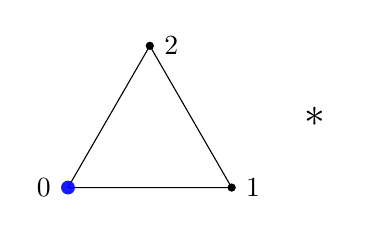
\begin{tikzpicture}[scale=.6]
\coordinate (A) at (210:2);
\coordinate (B) at (-30:2);
\coordinate (C) at (90:2);

\draw[draw=black] (A) -- (B) -- (C) -- (A);

\node[circle,fill=blue, opacity=.9, inner sep=0pt,minimum size=5pt, label=left:{0}] (a) at (A) {};
\node[circle,fill=black,inner sep=0pt,minimum size=3pt, label=right:{$1$}] (a) at (B) {};
\node[circle,fill=black,inner sep=0pt,minimum size=3pt, label=right:{$2$}] (a) at (C) {};

\node[scale=1.5] at (3.5,0.5) {$\ast$};
\end{tikzpicture}
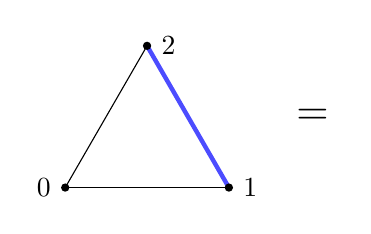
\begin{tikzpicture}[scale=.6]
\coordinate (A) at (210:2);
\coordinate (B) at (-30:2);
\coordinate (C) at (90:2);

\draw[draw=blue,  ultra thick, draw opacity=.7] (B) -- (C);
\draw[draw=black] (C) -- (A);
\draw[draw=black] (A) -- (B);

\node[circle,fill=black,inner sep=0pt,minimum size=3pt, label=left:{$0$}] (a) at (A) {};
\node[circle,fill=black,inner sep=0pt,minimum size=3pt, label=right:{$1$}] (a) at (B) {};
\node[circle,fill=black,inner sep=0pt,minimum size=3pt, label=right:{$2$}] (a) at (C) {};

\node[scale=1.5] at (3.5,.5) {=};
\end{tikzpicture}
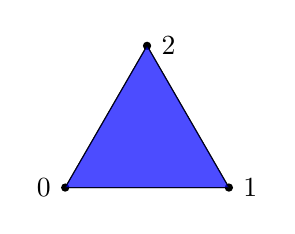
\begin{tikzpicture}[scale=.6]
\coordinate (A) at (210:2);
\coordinate (B) at (-30:2);
\coordinate (C) at (90:2);

\draw[draw=black] (A) -- (B) -- (C) -- (A);

\node[circle,fill=black,inner sep=0pt,minimum size=3pt, label=left:{$0$}] (a) at (A) {};
\node[circle,fill=black,inner sep=0pt,minimum size=3pt, label=right:{$1$}] (a) at (B) {};
\node[circle,fill=black,inner sep=0pt,minimum size=3pt, label=right:{$2$}] (a) at (C) {};

\draw[draw, fill=blue, opacity=.7] (A) -- (B) -- (C) -- (A);
\end{tikzpicture}}}
%
%	\medskip\pause
%
%	\only<6>{Also, versions for: \par
%		\qquad \textcolor{pblue}{cubical} (Kaufmann--Med.) and \par
%		\qquad \textcolor{pblue}{multisimplicial} (Med.--Pizzi--Salvatore) chains.}
%\end{frame}

\begin{frame}[fragile]{Cup-$(p,i)$ structures}

	\vskip-5pt\pause

	\begin{block}{Construction (Kaufmann-Med.)}
		Explicit May--Steenrod structures defining \textcolor{pblue}{operations} on $H^\bullet(-; \Fp)$.
	\end{block}

	\pause

	\begin{block}{Implementation (Med.)}
		In the computer algebra system \verb|ComCH|.
	\end{block}

	\pause

	For example, $\Delta_{3,2}[0,1,2]$ is equal to

	\begin{verbatim}
		- [0,1][0,1,2][0,1] + [0,1,2][0,2][0,1] + [0,2][0,2][0,1,2]
		- [0,1,2][0,1,2][1] - [0,2][0,1,2][1,2] + [0,1,2][1,2][1,2]
		- [0,1][1,2][0,1,2] - [0,1,2][2][0,1,2] - [0][0,1,2][0,1,2]
	\end{verbatim}

	\pause

	\textcolor{pblue}{Future directions:}

	\pause
	\begin{enumerate}
		\item Faster implementations for use in TDA. \pause \\
		\item Relation to higher category theory. \pause \\
		\item Connections to convex geometry. \pause \\
		\item Cartan and Adem coboundaries. \pause \\
		\item Where are these used in physics?
	\end{enumerate}
\end{frame}